% Chapter 2
\chapter{پیش زمینه و مروری بر مطالعات انجام شده}

رشد چشمگیر فناوری به همراه سهولت دسترسی به اینترنت در سال‌های اخیر باعث شده که بیشتر دستگاه‌های اطراف خود را متصل به اینترنت ببینیم. این دنیای جدید که به دنیای اینترنت اشیاء معروف است شامل خانه‌های هوشمند، دستگاه‌های پوشیدنی، خودروهای خودران و تلفن‌های هوشمند و... است که همگی زندگی روزمره انسان را تغییر داده‌اند. استفاده از این سیستم‌ها همگی باعث تولید حجم قابل توجهی داده در طول روز می‌شود که شرکت‌های بزرگ فناوری از این داده‌ها بهره برده و با استفاده از آن‌ها اقدام به انواع سرویس‌دهی به کاربران خود می‌نمایند\cite{b8}. شرکت‌های پیشرو برای تصمیم‌گیری‌های کلان مدیریتی و ارائه سرویس بهتر و با کیفیت‌تر به مشتریان، نیازمند استفاده از مدل‌های هوش‌مصنوعی برای ارتقاء کیفیت سیستم‌های هوشمند خود در جهت بهره‌برداری از این داده‌ها هستند. روش‌های متنوعی در رابطه با نحوه استفاده از این مدل‌ها وجود دارد. در ادامه روش‌های مختلفی از مطرح‌ترین روش‌ها توضیح داده می‌شود و نگاهی ریز بینانه‌تر به یادگیری فدرال و رابطه‌ آن با اینترنت اشیاء انداخته می‌شود\cite{ref5}.

\section{نگاه نزدیک‌تر به الگوریتم‌های یادگیری}

با توجه به رشد علم هوش مصنوعی و استفاده از روش‌های یادگیری ماشین، می‌توان از حجم بسیار زیاد داده تولید شده توسط گره‌های اینترنت اشیاء به نحو مطلوبی استفاده نمود و الگوریتم‌های مورد نظر، جهت رسیدن به اهداف مختلف را بر روی آن‌ها اجرا کرد. حال برای مدیریت و اجرای الگوریتم‌های یادگیری، روش‌های مختلفی وجود دارد که به توضیح هر یک از آن‌ها خواهیم پرداخت.

\subsection{یادگیری متمرکز}

این روش که در اکثر سیستم‌های حال حاضر امروزی مورد استفاده قرار می‌گیرد به این نحو است که تمام گره‌ها اطلاعات موجود خود را به صورت کامل به سیستم سرویس‌دهنده ابری ارسال می‌نمایند و سرویس‌دهنده ابری در حالی که تمام داده‌ها را در اختیار دارد، اقدام به اجرای الگوریتم‌های مورد نظر می‌کند. در شکل \ref{centralized} این روش به نمایش گذاشته شده است.

    \begin{figure}[H]
      \centering
      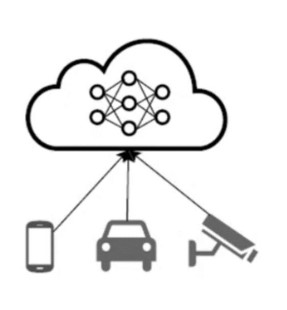
\includegraphics[height=4cm,width=6cm]{./types of ML/centralized .jpg}
      \caption[یادگیری متمرکز]{ یادگیری متمرکز\cite{ref6}}
      \label{centralized}
      \centering
    \end{figure}

سیستم‌های متمرکز تا پیش از این، اکثر نیازهای مربوطه را برطرف نموده‌اند ولی در دنیای امروزی و با توجه به زیاد شدن هر روزه دستگاه‌های متصل، موارد دیگری نیز مورد توجه واقع شده است. هزینه‌های ارتباطی ارسال حجم وسیع داده از یک سمت و نگرانی‌ها حول انتقال اطلاعات حساس و شخصی از سمت دیگر، توجه محققان را به سمت الگوریتم‌های غیر متمرکز و توزیع شده در یادگیری ماشین سوق داده است.

این روش دارای نقاط قوت و ضعف مختلفی است. از نقاط قوت این روش می‌توان به سرعت و دقت بالا، همگام‌سازی و یکنواختی داده‌ها و حفاظت و امنیت بالای داده‌ها اشاره کرد. از نقاط ضعف این روش می‌توان به وابستگی به هزینه و پایداری سرویس دهنده ابری، حساسیت به حجم و نوع داده‌های منتقل شده و چالش برانگیزی در برابر تغییرات محیط ذکر کرد. این روش در بسیاری از سرویس‌های آنلاین مورد استفاده قرار می‌گیرد.

\subsection{یادگیری غیرمتمرکز}

    در این روش هر گره به صورت مجزا اقدام به اجرای الگوریتم‌های مورد نظر می‌کند و در واقع پس از اجرای چند مرحله از کد، اطلاعات به‌روز شده را با گره‌های همسایه به اشتراک می‌گذارد. این کار به قدری ادامه پیدا می‌کند تا همگی به مقدار تعیین شده همگرا شوند. در شکل \ref{decentralized} این روش به نمایش گذاشته شده است.

    \begin{figure}[H]
      \centering
      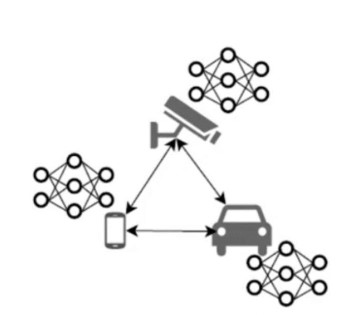
\includegraphics[height=4cm,width=6cm]{./types of ML/decentralized .jpg}
      \caption[یادگیری غیر متمرکز]{ یادگیری غیر متمرکز\cite{ref6}}
      \label{decentralized}
      \centering
    \end{figure}

 از مزایا و معایب این روش یادگیری این است که به گره‌ها اجازه می‌دهد که با توجه به شرایط و پارامتر‌های محلی خود، الگوریتم‌های خود را اجرا، تنظیم و بهینه‌سازی کنند. این روش همچنین باعث می‌شود که بار پردازشی و هزینه انتقال داده‌ها کاهش یابد و حریم خصوصی و حفاظت از داده‌ها حفظ شود. اما این روش نیز دارای چالش‌هایی است. از جمله سرعت و دقت پایین‌تر در پردازش داده‌ها، ناهمگام‌سازی و نامنظم بودن داده‌ها بین گره‌ها و نیاز به تضمین و تأیید صحت و کامل بودن داده‌ها. این روش در برخی از سیستم‌های آنلاین مانند بیت‌کوین\LTRfootnote{Bitcoin} و تورنت\LTRfootnote{Torrent} مورد استفاده قرار می‌گیرد.

\subsection{یادگیری توزیع شده}

    در این روش، مدیریت کل سیستم و تمام داده‌ها در اختیار یک هسته مرکزی قرار دارد ولی به دلیل نیاز به توان پردازشی بالا، این هسته بار پردازشی را بین گره‌های موجود تقسیم می‌کند. در ابتدای راه یادگیری توزیع شده، فرض بر این بوده است که تمام گره‌ها توان پردازشی یکسانی داشته و داده‌ها به میزان مساوی بین گره‌ها پخش خواهند شد. در شکل \ref{distributed} این روش به نمایش گذاشته شده است.

    \begin{figure}[H]
      \centering
      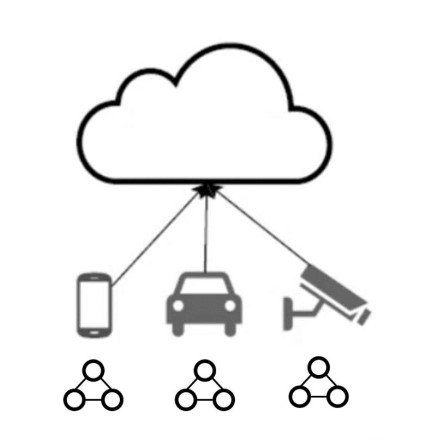
\includegraphics[height=4cm,width=6cm]{./types of ML/distributed .jpg}
      \caption[یادگیری توزیع شده]{ یادگیری توزیع شده\cite{ref6}}
      \label{distributed}
      \centering
    \end{figure}


\subsection{یادگیری فدرال}
    همان‌طور که در فصل اول اشاره شد، در یادگیری فدرال بر خلاف روش‌های متمرکز یادگیری ماشین، تحلیل داده‌ها به دستگاه‌های لبه، گره و یا سرور گیرنده منتقل می‌شود. یادگیری فدرال راه‌حلی مطلوب برای مدل‌سازی داده‌ها در تعداد زیادی دستگاه کارگر است. در این چارچوب، به جای ارسال داده‌های خام، پارامترهای مدل‌های محلی در هر گام آموزش به سرور منتقل می‌شود. در شکل \ref{federal} این روش به نمایش گذاشته شده است.
    سرور در حقیقت نقش رهبری را ایفا می‌کند و با توجه به نوع داده‌ها، یا مدل شبکه عصبی ایجاد کرده و آن را به سمت کاربران ارسال می‌کند. حال کاربران با توجه به داده‌های خود شبکه را آموزش می‌دهند و بعد از چند بار تکرار، وزن‌های به‌روزرسانی شده را به سمت سرور بر می‌گردانند. همان‌طور که در شکل \ref{federal} مشاهده می‌شود، داده‌ها همگی در سمت کاربر قرار گرفته‌اند و به سمت سرور ارسال نمی‌شوند. عدم ارسال بخش اطلاعات گره‌ها در یادگیری فدرال، حفظ حریم شخصی کاربران را ارتقا می‌بخشد.
    \begin{figure}[H] \centering
      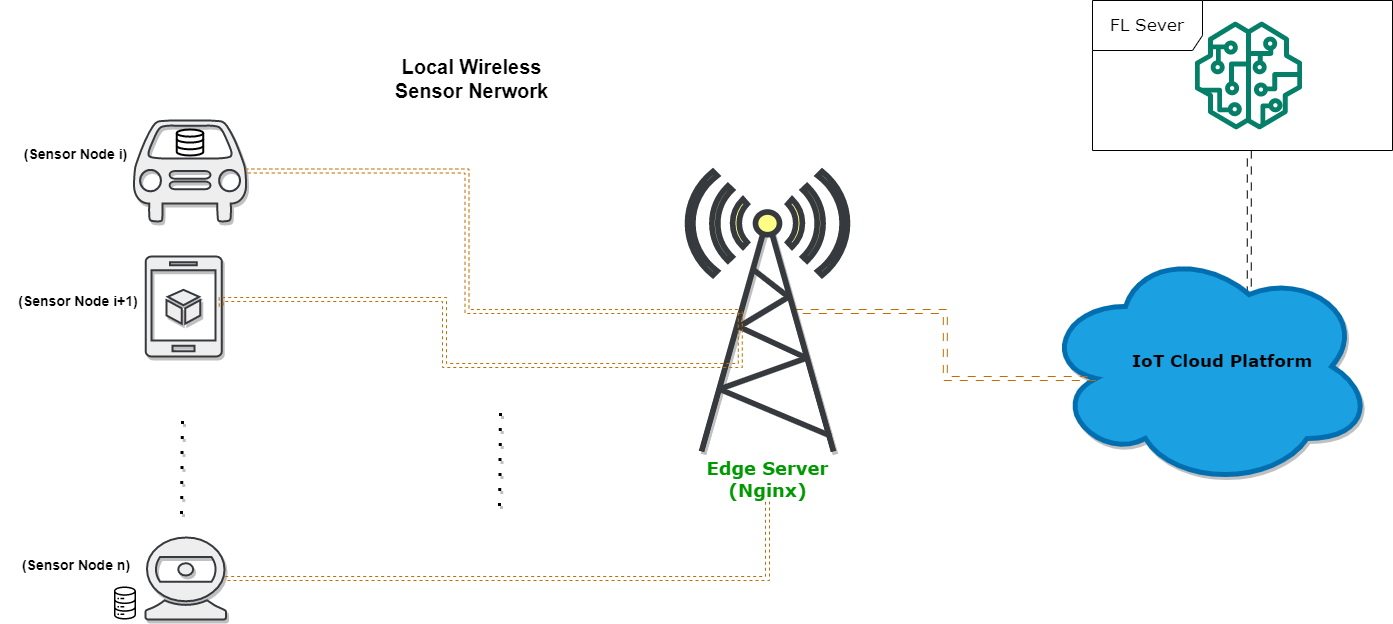
\includegraphics[height=8cm,width=15cm]{./IoT/State Diagram-Inter-connection.drawio.png}
      \caption{ شمایی از یادگیری فدرال در اینترنت اشیاء}
      \label{federal}
      \centering \end{figure}



      معمولاً برای تخمین و سنجش عملکرد روش‌های یادگیری ماشینی از مدل‌های شبکه عصبی استفاده می‌شود که کاربرد وسیعی در اکثر زمینه‌ها مانند پردازش تصویر، دسته بندی، پیش‌بینی و غیره دارند. امروزه با آمدن روش‌هایی آموزش و توسعه این روش‌ را از همیشه ساده‌تر شده است. علی‌رغم وجود مدل‌های گوناگون به عنوان مدل سراسری در یادگیری فدرال، اکثر استفاده‌های آن معطوف به مدل شبکه عصبی و به طور خاص‌تر شبکه‌های عصبی عمیق\LTRfootnote{Deep Neural Network} در پردازش تصویر به عنوان یکی از الزامات اساسی در اینترنت اشیاء می‌باشد. البته باید قبول کرد که در دسترس بودن و سادگی کار با آن‌ها نیز از دیگر عوامل روی‌ آوردن به آن‌ها می‌باشد. در ادامه به یکی از مطرح‌ترین استفاده از این مدل‌های دسته بندی کننده می‌پردازیم.



\subsection{الگوریتم FedAVG }

      از مطرح‌ترین و ساده‌ترین روش‌های ادغام کردن پارامتر‌های ارسالی (به عنوان مثال وزن‌ها و بایاس‌های شبکه عصبی) توسط تجمیع کننده الگوریتم میان‌گیری از آن‌ها با وزن یکسان بین تمامی کارگران می‌باشد. این الگوریتم با نام \lr{Federated Averaging} برای اولین بار در \cite{b6} مطرح شده است. در نسخه‌های اولیه یادگیری فدرال، این الگوریتم به صورت متمرکز درون تجمیع کننده در انتهای هر دور از یادگیری اجرا می‌شود تا در نهایت تمام کارگران با وزن یکسان در فرآیند یادگیری سهیم باشند. در ادامه شبه‌کد دو تکه اصلی مورد نیاز از اجرای این الگوریتم در تجمیع‌کننده و کارگران آورده شده است.
      
      
      از مهم‌ترین ایراداتی که می‌توان به این نوع الگوریتم گرفت این است که به علت ناهمگونی داده‌ها بین کارگران نباید در میانگین‌گیری وزن یکسانی به آنها داد. به همین دلیل طی سال‌های اخیرمدل‌های پیشرفته‌تری از این استراتژی معرفی شده است\cite{ref4}.
      
      
      \begin{algorithm}[H]
          \caption{بروزرسانی مشترک: اجرا در هر کارگر}
          \label{alg:client_update}
          \begin{algorithmic}[1]
              \State \textbf{ورودی:} بردار وزن مدل $w$، (\lr{Local Mini Batch})اندازه دسته‌های کوچک محلی $B$
              \State \textbf{خروجی:} بردار وزن مدل به‌روزشده $w'$
              
              \Function{بروزرسانی-مشترک}{$w, B$}
                  \State تقسیم $P_k$ به دسته‌هایی به اندازه $B$: $بچها \gets \text{تقسیم\_به\_بچها}(P_k, B)$
                  
                  \For{$i = 1$ تا $E$} \Comment{عبورهای آموزشی محلی}
                      \For{$هر دسته$ در $دسته‌ها$}
                          \State $w \gets w - \eta \cdot \nabla f(w,دسته)$ \Comment{بروزرسانی وزن‌های مدل}
                      \EndFor
                  \EndFor
                  
                  \State \Return $w$
              \EndFunction
          \end{algorithmic}
      \end{algorithm}
      
      \begin{algorithm}[H]
          \caption{میانگین‌گیری مشترک: اجرا در سرور}
          \label{alg:federated_averaging}
          \begin{algorithmic}[1]
              \State \textbf{ورودی:} نرخ یادگیری جهانی $\eta$، تعداد کارگر‌ها در هر دور $C$، تعداد عبور آموزشی محلی $E$، اندازه مینی‌بچ محلی $B$
              \State \textbf{خروجی:} بردار وزن مدل میانگین $w_{\text{avg}}$
              
              \Function{میانگین‌گیری-مشترک}{$\eta, C, E, B$}
                  \State مقداردهی اولیه بردار وزن مدل: $w \gets w_0$
                  
                  \For{$t = 1$ تا $\infty$} \Comment{دوره‌های آموزشی}
                      \State انتخاب به صورت تصادفی $C$ کارگر: $کارگر‌های\_انتخاب‌شده \gets \text{انتخاب\_کارگر‌ها}(C)$
                      
                      \For{$k$ در $کارگر‌های\_انتخاب‌شده$}
                          \State انجام بروزرسانی مشترک برای کارگر $k$: $w_k \gets \text{بروزرسانی-مشترک}(w, B)$
                          \State بروزرسانی بردار وزن مدل برای کارگر $k$: $w \gets \text{تجمیع\_وزن‌ها}(w, w_k)$
                      \EndFor
                      
                      \State محاسبه میانگین وزن‌های تمام کارگر‌ها: $w_{\text{avg}} \gets \text{محاسبه\_میانگین\_وزن‌ها}(w, C)$
                  \EndFor
                  
                  \State \Return $w_{\text{avg}}$
              \EndFunction
          \end{algorithmic}
      \end{algorithm}
      
\section{شبکه عصبی کانولوشنی}
مدل ‌کردن پردازش‌هایی که انسان قادر به انجام آن بر روی تصاویر است (برای مثال تشخیص هویت با استفاده از حس بینایی) با یک برنامه کامپیوتری از دستاورد‌های چندین ساله محققین حوزه تصویر بوده است. با معرفی بخش‌بندی معنایی\LTRfootnote{Semantic Segmentation } و شبکه‌های عمیق تصور شد که این مشکلات با استفاده از این روش جدید قابل حل‌شدن هستند. ولی مشکل بزرگ در مسیر استفادهٔ شبکه‌های عمیق برای پردازش تصاویر، هزینهٔ محاسبات این روش برای استفاده بر روی حجم زیاد داده‌ای که یک تصویر را تشکیل می‌دهد است. در حالت متداول شبکه‌های عمیق برای محاسبهٔ مقدار خروجی هر نورون، خروجی تمام نورون‌های لایهٔ قبل استفاده می‌شود و شیوهٔ استفاده از خروجی هر یک از نورون‌های قبل با یک پارامتر مشخص می‌شود. یک تصویر نمونه با تراکم پیکسلی نسبتاً کم، برای مثال 256 × 256 را می‌توان به صورت یک بردار به طول 65536 در نظر گرفت. باتوجه‌به نحوه پیچیدگی شبکه‌های عصبی عمیق می‌توان درک کرد که حرکت داده‌ای با این حجم در لایه‌های یک شبکه عمیق می‌تواند به چه اندازه از نظر محاسبات سخت و سنگین باشد.

\begin{figure}[H]
  \centering
  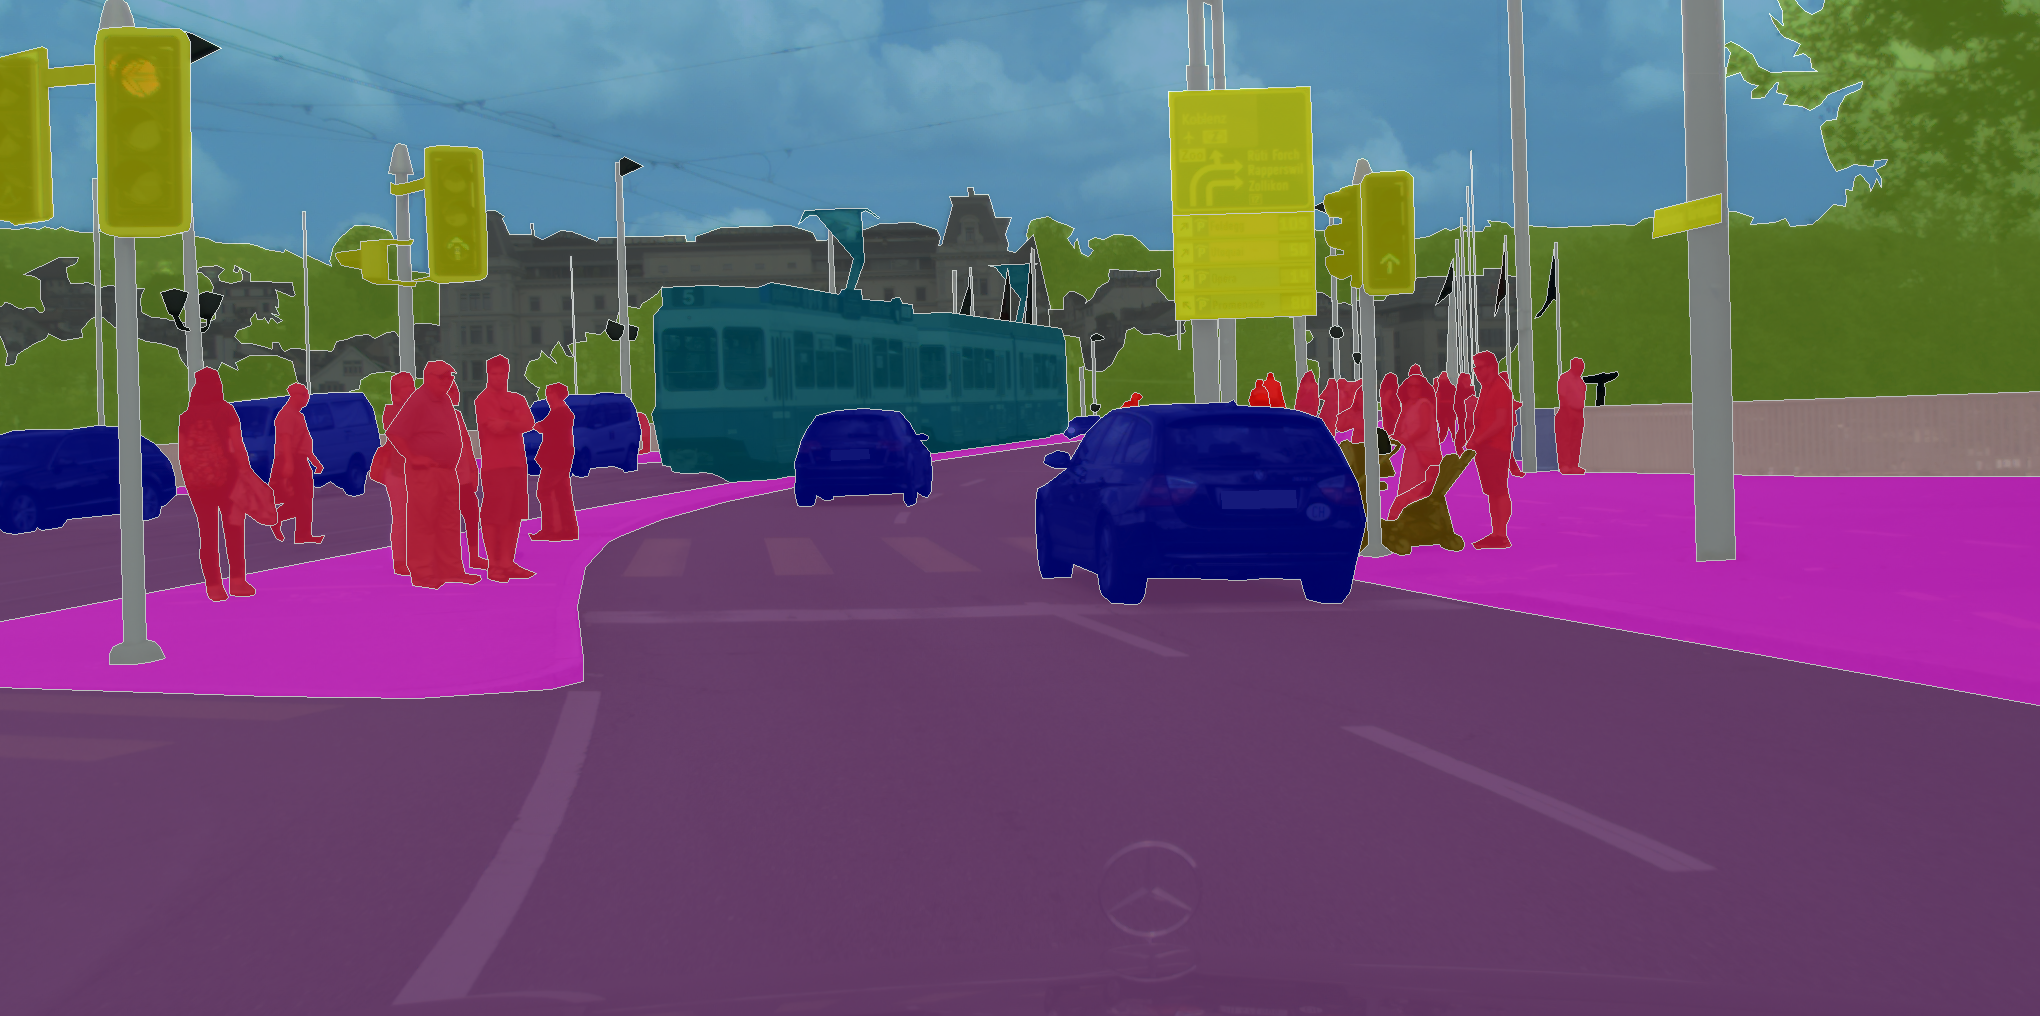
\includegraphics[height=8cm,width=12cm]{CNN/Zurich-Cityscapes.png}
  \caption[نمونه ی بخش بندی معنایی در ماشین های خودران]{ نمونه ی بخش بندی معنایی در ماشین های خودران\cite{ref7}}
  \label{CNN2}
  \centering
\end{figure}

برای عبور از این مانع، شبکه‌ای جدید با محوریت پردازش داده‌های تصویری (به‌ طورکلی تر پردازش سیگنال) طراح شد و این الگوریتم جدید را شبکه‌های عصبی کانولوشن\LTRfootnote{Convolutional Neural Networks } نام‌گذاری کردند. ایده اصلی این طرح جدید در این نکته بود که بهتر است برای محاسبهٔ خروجی هر نورون از خروجی تمام نورون‌های لایهٔ قبل استفاده نشود؛ بلکه کافی است فقط از همسایگان محدود از نورون‌های همسایه استفاده شود. در نتیجه هزینهٔ محاسبات برای پردازش و مهم‌تر از آن تعداد پارامترهای مدل کاهش می‌یابد. هر لایه از این شبکه (در ساده‌ترین حالت) با یک کرنل تعریف می‌شود که مقادیر آن به‌عنوان پارامترهایی قابل تغییر فرض می‌شود که شبکه در طول فرآیند یادگیری آنها را تنظیم می‌کند. ورودی هر لایهٔ تصویر (به‌عبارت ‌دیگر نقشهٔ ویژگی) و خروجی آن نیز به همین ترتیب است؛ ولی لزوماً رزولوشن این دو یکسان نیست. این کرنل بر روی تک‌تک پیکسل‌های تصویر اعمال می‌شود و تصویر خروجی تولید می‌شود. به این عملیات فیلتر کردن در شبکهٔ عصبی کانولوشن می‌گویند. در شکل \ref{CNN} معماری یک شبکه کانولوشن به عنوان نمونه آورده شده است.

\begin{figure}[H]
  \centering
  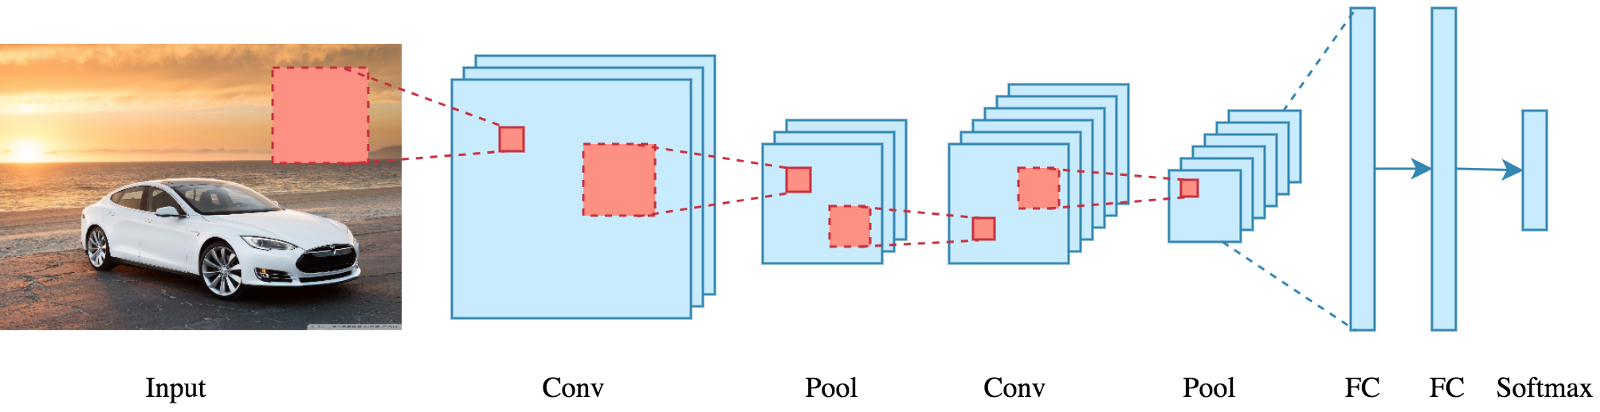
\includegraphics[height=5cm,width=15cm]{CNN/183560_qcMBDPuKpDvICcdd.png}
  \caption{ معماری یک شبکه کانولوشنی}
  \label{CNN}
  \centering
\end{figure}

این شبکه پس از معرفی توانست محبوبیت خاصی را بین محققان به دست آورد و همچنین مقدمه‌ای بر ساخت انواع پیشرفته‌تر از شبکه‌های عصبی برای عملیات مختلفی مانند تشخیص و شناسایی چهره\LTRfootnote{Face Recognition}، بخش‌بندی معنایی تصویر، تشخیص اشیاء، دسته‌بندی و گروه‌بندی تصاویر و غیره بشود.\cite{ref8}
\section{پردازش لبه}

در روش‌های مبتنی بر الگوی ابری، داده‌ها باید از طریق اینترنت برای یک مرکز داده متمرکز ارسال شود تا در آن‌جا پردازش شوند و نتیجه برای منبع بازگردانده شود. این روش برای حجم محدود و مشخصی از داده‌ها عملکرد خوبی دارد، اما هنگامی که حجم عظیمی از داده‌ها قرار باشد برای مراکز داده ارسال شود، در آن‌جا پردازش شود و نتیجه برای منبع بازگردانده شود مناسب نیست. زیرا نیاز به پهنای باند زیاد وجود دارد که مقرون‌به‌صرفه نیست. هم‌چنین مشکلات تاخیر و قطعی‌های غیرقابل پیش‌بینی شبکه، همگی می‌توانند باعث اختلال در عملکرد ارسال، دریافت و پردازش داده‌ها شوند. پژوهشگران برای حل این مشکل معماری پردازش لبه را ارائه کرده‌اند. پردازش لبه یک معماری توزیع‌شده است که در آن داده‌های کاربر در لبه شبکه و تا حد امکان نزدیک به دستگاه‌های انتهایی پردازش می‌شود. آمارها نشان می‌دهند که ساختار‌های مبتنی بر پردازش لبه در حال تغییر الگوی پردازش اطلاعات هستند و این احتمال وجود دارد که در آینده تغییرات مهمی در حوزه یادگیری به خصوص یادگیری‌های توزیع شده به وجود آورند\cite{edge1}.

در اصطلاح لبه شبکه به مکانی اشاره دارد که در آن داده‌ها تولید می‌شوند و تجهیزات محاسباتی در آنجا نصب شده‌اند. در محاسبات سنتی سازمانی، داده‌ها در سرورهای مرکزی ذخیره می‌شوند و از طریق شبکه محلی در اختیار کاربران قرار می‌گیرند. به عبارت دیگر، داده‌ها در زیرساخت‌های سازمانی ذخیره و پردازش شده و نتایج پردازش به کاربران ارسال می‌شود. این معماری بر اساس الگوی کلاینت و سرور است که بسیاری از برنامه‌های تجاری بر اساس آن عمل می‌کنند. با این حال، با پیدایش پردازش لبه، داده‌ها در نزدیک‌ترین مکان به منبع تولید آن‌ها پردازش شده و نتایج به کاربران ارسال می‌شود. این روش کمک می‌کند تا هزینه‌های ارتباطی کاهش یابد و حفظ حریم شخصی کاربران بهتر از قبل رعایت شود.

از آنجا که، تعداد دستگاه‌های متصل به اینترنت و حجم داده‌هایی که توسط دستگاه‌ها تولید می‌شوند و توسط کسب‌وکارها استفاده می‌شوند، فراتر از ظرفیت زیرساخت‌های مراکز داده سنتی است. یک مثال ساده در این زمینه، داده‌های تولیدشده در شبکه‌های اتومبیل‌های هوشمند است که به‌لحاظ تجاری و بازاریابی ارزش زیادی دارند و توسط خودرو تولید می‌شوند که عضو شبکه‌های اتومبیلی هستند. در سویی دیگر، داده‌های حساس‌به‌زمان وجود دارند که توسط تجهیزاتی مثل دوربین‌های نظارت تصویری ضبط می‌شوند و تصاویر از طریق اینترنت برای اپراتوری که مسئولیت نظارت بر دوربین‌ها را برعهده دارد ارسال می‌شود تا اگر مورد مشکوکی بود، اپراتور واکنش لازم را انجام دهد. در این روش نه‌تنها به پهنای باند زیادی برای ارسال داده‌ها نیاز است، بلکه باید اپراتور به‌سرعت به موارد مشکوک واکنش نشان دهد. حال اگر داده‌های تصویری به‌ شکل محلی توسط الگوریتم‌های هوشمند تحلیل شده و موارد مشکوک در قالب یک پیام متنی ساده برای اپراتور ارسال شود، به میزان قابل توجهی در پهنای باند صرفه‌جویی انجام می‌شود و زمان پاسخ‌گویی به رخدادها نیز کاهش پیدا می‌کند. در این حالت، فشار مضاعف بر اینترنت یا شبکه‌های گسترده وارد نمی‌شود و با مشکل ازدحام\LTRfootnote{Congestion} و اختلال\LTRfootnote{Disruption} روبه‌رو نخواهد شد.

\begin{figure}[H]
  \centering
  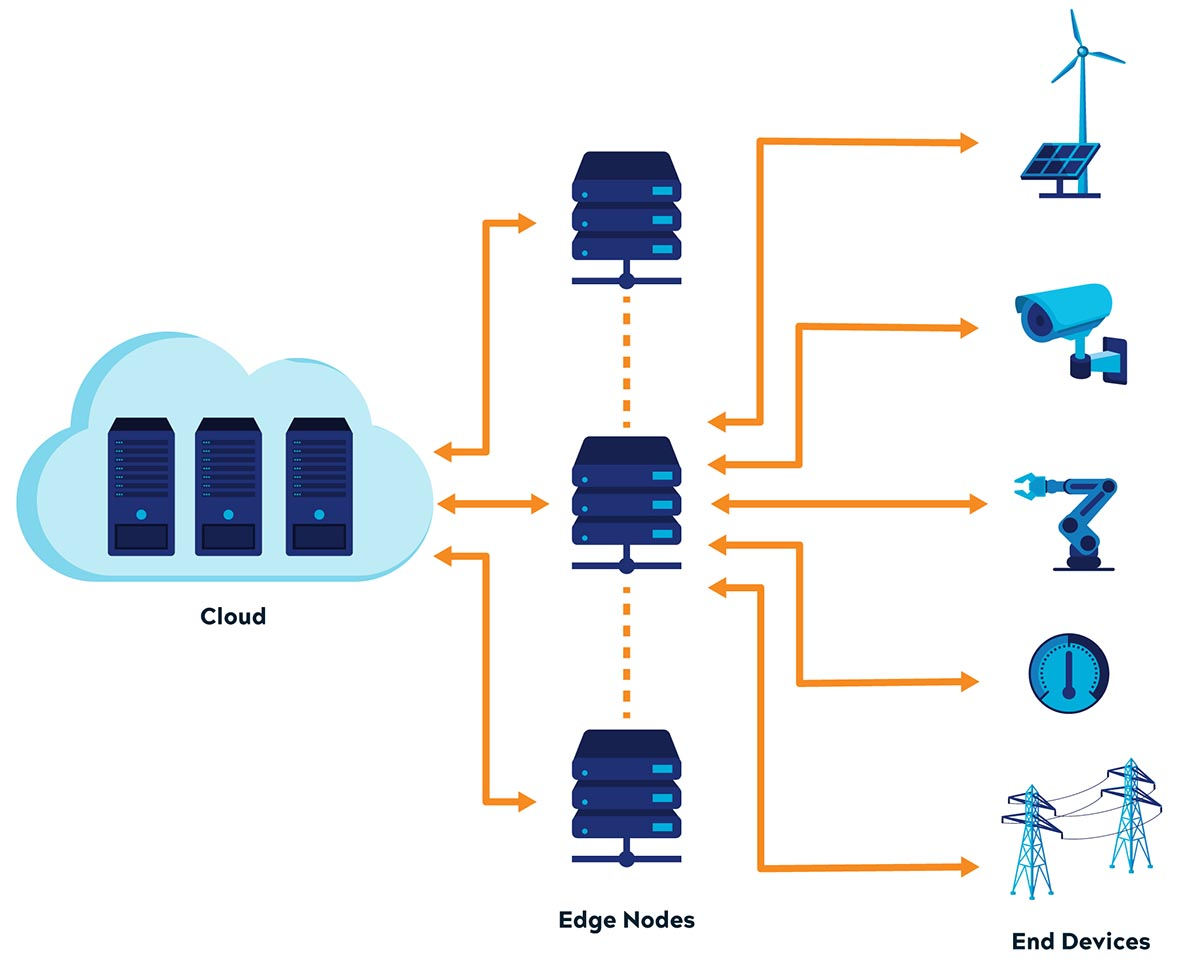
\includegraphics[height=8cm,width=13cm]{Edge/edge-computing-diagram.jpg}
  \caption{ دیاگرام یک شبکه دارای پردازش لبه}
  \label{Edge}
  \centering
\end{figure}

همین مسئله باعث شده تا معماران شبکه‌های کامپیوتری به‌جای طراحی مراکز داده متمرکز، به‌سراغ طراحی‌های مبتنی بر الگوی پردازش لبه بروند. به‌طوری‌که منابع ذخیره‌سازی و محاسباتی از مرکز داده به مکانی انتقال داده شود که نزدیک به منبع تولیدکننده داده‌ها است. دانستن این موضوع جالب خالی از لطف نیست که پردازش لبه بر مبنای یک تئوری خیلی ساده شکل گرفته است، اگر نمی‌توانید داده‌ها را به مرکز داده نزدیک کنید\cite{edge2}، مرکز داده را به داده‌ها نزدیک کنید.

\subsection{معماری‌های متنوع پردازش لبه}

همان‌طور که در شکل \ref{edge_arch} آمده است، می‌توان معماری‌های متنوعی برای حضور سرور لبه در شبکهٔ اینترنت اشیاء متصور شد. بسته به کاربرد و محل فیزیکی دستگاه‌ها می‌توان یکی از این معماری‌ها را برگزید. در این پروژه به دلیل ساده‌تر بودن و فراگیر بودن در کاربرد از معماری سلسله مراتبی استفاده شده است.

\begin{figure}[H]
  \centering
  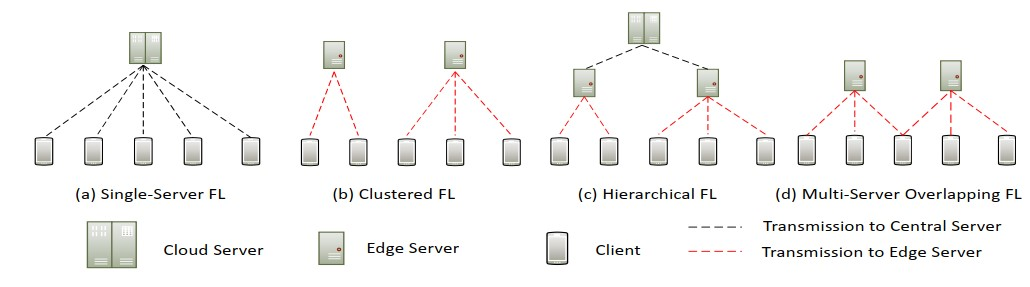
\includegraphics[height=7cm,width=15cm]{./arch/edge.jpg}
  \caption[انواع قرار گیری المان‌های اصلی در شبکه اینترنت اشیاء]{ انواع قرار گیری المان‌های اصلی در شبکه اینترنت اشیاء\cite{a10}}
  \label{edge_arch}
  \centering
\end{figure}

\section{یادگیری فدرال در اینترنت اشیاء}

شبکه‌های نوظهور اینترنت اشیا همچون دستگاه‌های پوشیدنی، خودروهای خودران یا خانه‌های هوشمند شامل تعداد بسیار زیادی حسگر هستند. این حسگرها توانایی جمع‌آوری عکس‌العمل و سازگاری با داده‌ها برای کاربرد بی‌درنگ را برای دستگاه‌های اینترنت اشیا فراهم می‌سازند. به عنوان مثال، خودروهای خودران به منظور عملکرد صحیح نیازمند یک مدل به روز از ترافیک شهری، اماکن و رفتار افراد پیاده هستند که این داده‌ها را از حسگرها دریافت می‌کند. ساخت مدلی سراسری در این حوزه به دلیل عدم تمایل افراد به در اختیار گذاشتن اطلاعات فردی، مانند اطلاعات مکانی و محدودیت در ارتباطات هر دستگاه بسیار مشکل است. از این رو، روش‌های یادگیری فدرال می‌توانند مدلی سازگار با تغییرات ایجاد نمایند و این سیستم‌ها را در عین حفظ حریم شخصی به خوبی آموزش دهند. شکل \ref{iot} بیانگر تنها بخشی از حوزه‌هایی است که در آینده‌ای نه چندان دور از ترکیب این دو حوزه به وجود می‌آید.
\begin{figure}[H]
  \centering
  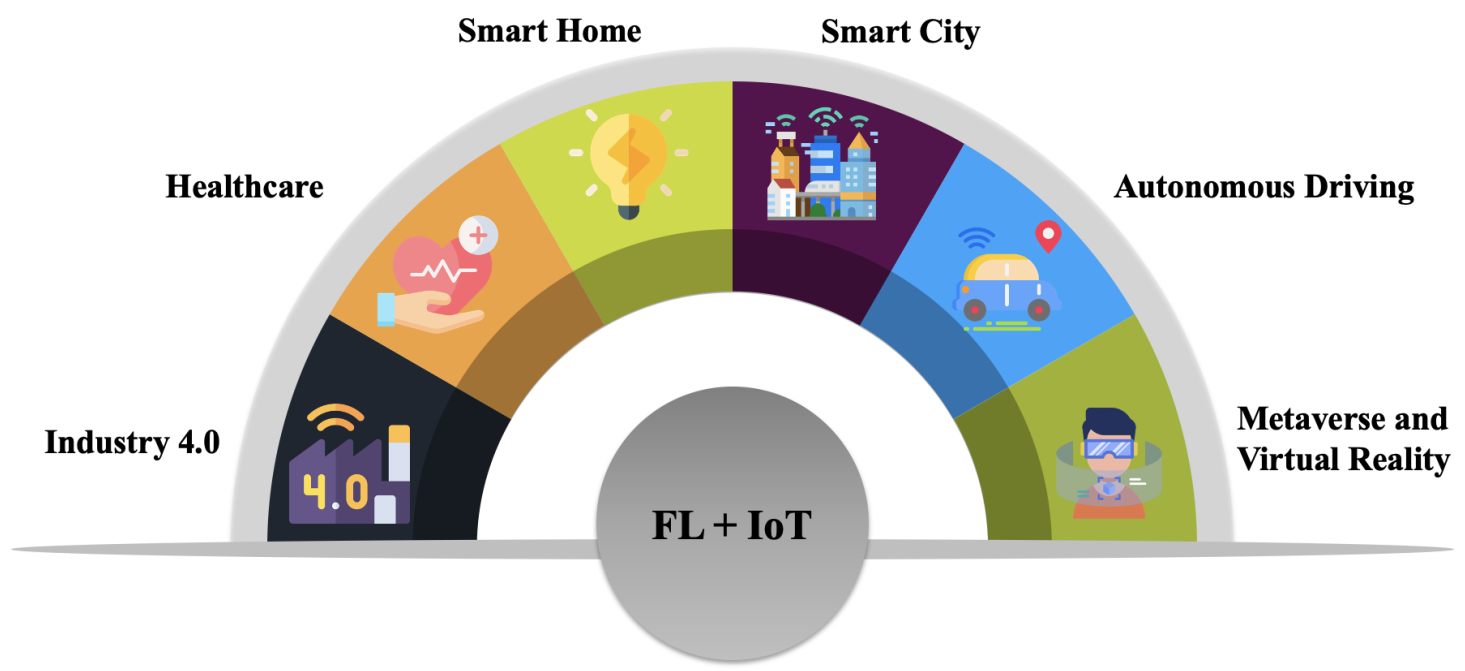
\includegraphics[height=7cm,width=13cm]{./IoT/IOT.png}
  \caption[کاربرد‌های یادگیری فدرال در اینترنت اشیاء]{ کاربرد‌های یادگیری فدرال در اینترنت اشیاء\cite{a10}}
  \label{iot}
  \centering
\end{figure}

\section{جمع بندی}
ایجاد بستری که تمامی موارد بالا در آن نقش پررنگی ایفا می‌کنند، می‌تواند محیط خوبی برای توسعه برنامه‌های مختلف با توجه به نیازهای کاربر باشد. این پروژه تنها بخشی از این نیاز‌ها را پوشش می‌دهد که کاربرد نسبتاً بالایی در دسته‌بندی تصاویر را ارائه می‌کند. در اینجا، سعی می‌شود با استفاده از ساده‌سازی‌های صورت گرفته، به تأکید بر پیاده‌سازی سیستمی که از یادگیری فدرال بهره می‌برد پرداخته شود. در نهایت با توجه دانش قبلی در مورد موارد ذکر شده در این فصل و بهره‌گیری از شبیه‌سازی‌های متنوع، به دسته‌بندی داده‌های مجموعه داده CIFAR-10 با استفاده از یک شبکه عصبی کانولوشن روی یک بستر شبکه اینترنت اشیاء که در آن از پردازش لبه استفاده شده خواهیم پرداخت. در فصل بعدی به جزئیات بیشتر این شبیه‌سازی پرداخته می‌شود.
%%%%%%%%%%%%%%%%%%%%%%%%%%%%%
